\chapter{Implementation}
The following chapter will describe the choices and the inner workings of the project.
The implementation is divided in multiple parts (the text in fixed width font refers to the corresponding source code folder) : 

\begin{itemize}
\item An audio manipulation framework.
\item The implementation of many audio and watermarking algorithms, in this framework : the whole makes the library that we call \texttt{libwatermark}.
\item A test application to ensure correctness of the library : \texttt{lib\_testapp}.
\item A graphical interface that uses the library : \texttt{InterfaceWatermarking}.
\end{itemize}

All of these parts will be reviewed in the following sections. Theye are all thoroughly documented with \brand{Doxygen}, and the complete documentation can be found in the \texttt{doc} folder.

\section{Technologies used}
The choice was made really early to use \brand{C++} as a programming language, mostly because of the speed, but also because it is quite cross-platform. We also used many \brand{C++11} features for the sake of learning, and because it sometimes reduces the amount of code needed. However, on \brand{Microsoft Windows} with \brand{Visual Studio}, all the features might not be supported by the compiler.

\subsection{Dependencies}
We tried to use as few dependencies as possible, and we tried to choose the most cross-platform ones. In return, our software should work on every common desktop operating system, and could certainly be embedded in smartphones, etc\dots
\subsubsection{Qt}
The GUI framework. It is not used in the library, but it allowed us to make a fully working \ac{GUI} in a really short amount of time; also, most of us already had some prior knowledge of it.
\subsubsection{FFTW}
This Fast Fourier Transform library has been used as the main library to perform the Fourier transform needed in some algorithms, because of its efficiency. However, other \ac{FFT} libraries could be used very easily.
\subsubsection{libsndfile}
An audio file library that allows our software to open \brand{WAV} files and other common filetypes very easily. It is lightweight and efficient. Unfortunately, it doesn't support compressed formats like \brand{MP3} or \brand{OGG Vorbis}. 

\section{Framework}
An audio framework has been designed in order to streamline the audio processing operations and concentrate only on the algorithms.

The other alternatives would have been :
\begin{itemize}
\item To code every algorithm in its own function, with some helper functions to load a file, etc\dots which would have resulted in a lot less code but also a less reusable code.
\item To work in \brand{MATLAB}, which reduces the overhead needed since loading and saving files, as well as transforms, are already implemented.
\end{itemize}

A lot of effort went into making it very generic, fast, and reliable for any kind of audio operations.


\subsection{Operation}
The main idea is : 
\begin{enumerate}
\item To load some audio data.
\item To apply an algorithm to chunks (e.g. 512 samples for instance) of this data.
\item To save the result if needed.
\end{enumerate}

For instance, on a 2048 samples audio file, with a buffer size of 512, there would be four buffers that would each see the algorithm applied to them.

In the current design, there is an input and an output, input and output filters, and the algorithm. For instance, here would be the call order of a generic example.

\begin{enumerate}
\item FFT plotting \textit{calls} FFT \textit{calls} GetNextBuffer
\item Algorithm
\item IFFT \textit{calls} Waveform plotting \textit{calls} WriteNextBuffer
\end{enumerate}

However, this is somewhat clumsy to setup : one must first instantiate the original audio loader I0, then the \ac{FFT} filter I1 which has to reference I0, then the plotter I2 which has to reference I1, and finally the manager class which has to reference I2, and the same for the output, which leads to bloated code and a logical dissimetry.
So in future project, the framework might be modified to take instead a list of classes which would make our example:

GetNextBuffer $\rightarrow$ FFT $\rightarrow$ FFT plotting $\rightarrow$ Algorithm $\rightarrow$ IFFT $\rightarrow$ Waveform Plotting $\rightarrow$ WriteNextBuffer.

\newpage

\subsection{Capabilities}
Since an heavy emphasis has been put into having very generic interfaces, we have been able to implement many useful features and algorithms.

The library is entirely templated, which means that most of the classes can be used with fixed or floating point numbers. However, it does not always make sense : for instance, \brand{FFTW} only works in floating point, so using \texttt{short int} as a base sample type would not work.

Multiple channels are supported in a seamless way, and can be interweaved or deinterweaved.

There are interfaces for : 
\begin{itemize}
\item Inputs and outputs \& filters.
\item Transforms.
\item Watermarking \& degradation algorithms.
\item Time management.
\item Watermark embedding.
\item Copying, overlapping and windowing.
\end{itemize}

\subsubsection{A short word on overlap-add processing}
This was by far one of the most difficult part of the library to get right, mainly due to the numerous interactions between different parameters and algorithms, and complexity of the subject.

The main process is explained on \cite{overlap}, however, one of the main point to take into account is the necessity of windows functions.

Since we aim for resynthesis, we have to select window functions that would sum to unity on at least one overlap factors as explained on \cite{smith1987parshl}, in the section "Choice of Hop Size". 

Several of these functions are shown in \cite{heinzel2002spectrum}, and some of theme are implemented. Since they are mostly high-order cosine windows, they can be implemented solely by inputting an array of values and an ideal overlap factor as shown on the file \texttt{libwatermark/io/fftproxy/window/HighOrderCosineWindow.h}.
\subsection{Feature list by class}
You can see on figures \ref{frameworkclass1} to \ref{frameworkclass4} tables that repertories all the implementations of these interfaces.

\begin{figure}[h!]
\centering
\begin{tabular}{|c|c|l|}
\hline
\textbf{Inputs} & \textbf{Outputs} & \textbf{Explanation} \\
\texttt{InputManagerBase} & \texttt{InputManagerBase}  & \\
\hline
FileInput & FileOutput & Wrapper around \brand{libsndfile} \\
BufferInput & BufferOutput & Read and write from a buffer \\
SilenceInput & DummyOutput & Generates silence and writes to nothing \\
\hline
FFTInputProxy & FFTOutputProxy & \ac{FFT} transform \\
MCLTInputProxy & MCLTOutputProxy & \ac{MCLT} transform \\
\hline
& GnuplotOutput & Displays sample data in \brand{GNUPlot} \\
& GnuplotFFTOutput & Displays a spectrum in \brand{GNUPlot} \\
\hline
\end{tabular}

\vspace{1em}

\begin{tabular}{|c|c|l|}
\hline
\textbf{Input copy handlers} & \textbf{Output copy handlers} &  \textbf{Explanation} \\
\texttt{InputCopy} & \texttt{OutputCopy} & \\
\hline
InputSimple & OutputSimple & Copies and increment by a buffer size \\
InputOLA & OuputOLA & Copies in an overlap-add fashion\\
InputFilter & OutputFilter & Copies in order to perform convolution \\
\hline
\end{tabular}

\vspace{1em}

\begin{tabular}{|c|l|}
\hline
\textbf{Window} & \textbf{Explanation} \\
\texttt{WindowBase} & \\
\hline
RectWindow & Rectangular window : does nothing \\
BartlettWindow & Bartlett window \\
HighOrderCosineWindow & Allows the conception of cosine windows like \\ & Hann, Hamming, Blackman, Nuttal, STxF  \\ 
\hline
\end{tabular}

\caption{Objects related to input-output}
\label{frameworkclass1}
\end{figure}

\begin{figure}[h!]
\centering
\begin{tabular}{|c|c|l|}
\hline
\textbf{Watermark encoding} & \textbf{Watermark decoding} & \textbf{Explanation} \\
\texttt{WatermarkBase} & \texttt{WatermarkBase} & \\
\hline
LSBEncode & LSBDecode & \ac{LSB} algorithm \\
RLSBEncode & RLSBDecode & Resistant \ac{LSB} algorithm \\
SSWEncode & SSWDecode & \ac{SSW} algorithm \\
\hline
\end{tabular}

\vspace{1em}

\begin{tabular}{|c|l|}
\hline
\textbf{Audio degradations} & \textbf{Explanation} \\
\texttt{BenchmarkBase} & \\
\hline
AddBrumm & Adds mains-like noise \\
AddWhiteNoise & Adds white noise \\
Amplify & A simple gain \\
Convolution & Performs linear convolution for filtering (e.g. LPF / HPF)\cite{convolution}\\
Exchange & Exchanges pairs of samples \\
FFTNoise & Adds white noise using a spectral method \\
FFTAmplify & Gain using a spectral method \\
Invert & Inverts the phase of the audio \\
Smooth & Smoothes the samples \\ 
Stat1 & Also smoothes the samples \\
ZeroCross & Strict noisegate\\
\hline
\end{tabular} 
\caption{Audio algorithms}
\label{frameworkclass2}
\end{figure}

\begin{figure}[h!]
\centering
\begin{tabular}{|c|l|}
\hline
\textbf{Time management} & \textbf{Explanation} \\
\texttt{TimeAdapter} & \\
\hline
AtTime & Starts the algorithm at a certain buffer \\
Every & Starts the algorithm every $k$ buffer \\
For & Starts the algorithm for $n$ buffers \\
Every\_For & Every $k$ buffers, starts the algorithm and stops it after $n$ buffers\\
\hline
\end{tabular}
\caption{Algorithm triggering}
\label{frameworkclass3}
\end{figure}

\begin{figure}[h!]
\centering
\begin{tabular}{|c|l|}
\hline
\textbf{Watermark embedding} & \textbf{Explanation} \\
\texttt{WatermarkData} & \\
\hline
SimpleWatermarkData & Puts the watermark a single time \\   
LoopingWatermarkData & Puts the watermark repeatedly \\
\hline
\end{tabular}
\caption{Watermarked data-related objects}
\label{frameworkclass4}
\end{figure}

Also, the folder \texttt{src/matlab} contains a \brand{MATLAB} implementation of the compression-expansion algorithm, that we could not port to \brand{C++} due to lack of time.

\newpage

\subsection{Class diagram}

The class diagram (figure \ref{classdiagram}) only shows child classes when it is relevant; else it would cause too much bloat.

Some important things to note are that :
\begin{itemize}
\item The class diagram shown here is for a generic instantiation with a watermark algorithm (it is very similar for an evaluation algorithm). 
\item Due to the complexity of the library, we will only show relevant public members and interfaces : detailed documentation is available thanks to \brand{Doxygen}.
\item Most of the classes do reference a \texttt{Parameters} class (figure \ref{parametersclass}) which holds some common parameters and types used across the library.
\item Most of the classes are templates with a \texttt{data\_type} parameter that can be \texttt{short}, \texttt{double}...
\end{itemize}


\begin{figure}[h!]
\centering
\begin{tikzpicture}
\umlclass[template=data\_type]
{Parameters}
{
	size\_type = unsigned long int \\
	complex\_type = complex<data\_type> \\
	samplingRate : size\_type \\
	bufferSize : size\_type \\	
}
{
	normFactor() : data\_type \\
}
\end{tikzpicture}

\caption{The Parameters class}
\label{parametersclass}
\end{figure}

\begin{figure}[h!]
\centering

\begin{tikzpicture}
% % % CLASS DIAGRAM HERE % % %
% Base Manager

\umlinterface[x=0,y=8]
{ManagerBase}
{}
{
	\umlvirt{prepare() : void} \\
	\umlvirt{execute() : void} \\
}

\umlclass[x=0,y=5]
{WatermarkManager}
{}
{
	\umlvirt{prepare() : void} \\
	\umlvirt{execute() : void} \\
}

% WatermarkBase
\umlinterface[x=0,y=2]{WatermarkBase}{}
{
	\umlvirt{operator()() : void} \\
}

% IO
\umlinterface[x=-6,y=6]{IOManagerBase}{}
{
	channels() : size\_type \\
	frames() : size\_type \\
	v() : vector<vector<data\_type>> \\
}
\umlinterface[x=-6,y=2]{InputManagerBase}{}
{
	getNextBuffer() : Buffer \\
}
\umlinterface[x=-5,y=-1]{OutputManagerBase}{}
{
	writeNextBuffer(Buffer) : void \\
}

% WM data
\umlinterface[x=5,y=7]{WatermarkData}{}
{
	setSize() : void\\
	nextBit() : bool\\
	setNextBit(Bool) : void \\
	isComplete() : bool \\
}

% TA
\umlinterface[x=6,y=2]{TimeAdapter}{}
{
addStartHandler(Function) : void\\
addStopHandler(Function) : void\\
perform() : void \\
}
% Links
\umlinherit{WatermarkManager}{ManagerBase}
\umlinherit{InputManagerBase}{IOManagerBase}
\umlinherit{OutputManagerBase}{IOManagerBase}

\umlaggreg{InputManagerBase}{WatermarkManager}
\umlaggreg{OutputManagerBase}{WatermarkManager}
\umlaggreg{WatermarkBase}{WatermarkManager}
\umlaggreg{WatermarkData}{WatermarkManager}
\umlaggreg{TimeAdapter}{WatermarkManager}

\end{tikzpicture}

\caption{Class diagram for the main usage of the framework}
\label{classdiagram}
\end{figure}

\newpage

\subsection{Example of usage}
We will here have a look at an example usage of our library which will correspond to the encoding of some bits with the \ac{LSB} algorithm.

More examples can be seen in the test application.

\begin{figure}[h!]
\centering

\begin{lstlisting}
    Parameters<short> conf;
    
    WatermarkData* data = new SimpleWatermarkData; // Set the bits afterwards 
    auto input = new FileInput<short>("input_mono.wav", conf);
    auto output = new FileOutput<short>(conf);

    auto algorithm = new LSBEncode<short>(conf);

    WatermarkManager manager(Input_p(input),
    						 Output_p(output),
    						 Watermark_p(new LSBEncode<short>(conf)),
    						 WatermarkData_p(data));
    manager.execute();

    output->writeFile("lsb_encode.wav");
\end{lstlisting}

\caption{Example instanciation}
\end{figure}

\newpage

\section{Algorithms}
\subsection{Watermarking and evaluation algorithms}
They are separated in two folders : \texttt{benchmark} and \texttt{watermark}.

We tried very hard to use the \brand{C++11} features efficiently in our code.

Here is for instance the code that performs the \texttt{Amplify} operation : 

\begin{figure}[ht!]
\centering
\begin{lstlisting}
			for(auto& sampleData : channelsData)
			{
				MathUtil::apply(sampleData,
				[&] (data_type x)
				{
					return x * _gain;
				});
			}
\end{lstlisting}
\caption{Amplify algorithm}
\label{amplify}
\end{figure}

It reads very easily : "For each channel, multiply the whole channel by the gain", thanks to lambda-expressions and range-based for-loops.

We also made our system so that the user of our framework can choose when does the effect starts, how long it should last, and if it repeats. The granularity is the buffer size.

For instance, in order to make some benchmarks, it is possible to make a volume modification using the algorithm on figure \ref{amplify} every 80 buffers, for 5 buffers, starting at 200 buffers.
\subsubsection{Details on the watermarking implementation}
There are some things to note about our implementation : 
\begin{itemize}
\item In case of multi-channel operation, the same bits are copied on each channel. But the algorithms are easily tweakable.
\item In our tests, most of the time, the watermark is only put at the beginning of the file. However, it could be put in a looping mode by a simple class change.
\item In order to be able to read data, the size of the watermark to read is embedded at the beginning, using the 64 first bits. However, if these bits are damaged, it can become impossible to get access to the other parts of the watermark because the algorithm won't know when to stop reading, which can cause buffer overflows.
\item There are a few bugs which could not be settled due to the lack of time : 
\begin{itemize}
\item In case of windowing in an overlap-add process, the first window would sometimes need to be normalized.
\item Since the output doesn't know about the input and only takes fixed-size buffers as input, if reading and writing a file, the output file might be a few bytes longer than the input file.
\end{itemize}
\end{itemize}
\subsection{Transforms}
The main problem with transforms is that they might be transforming from and to different domains.
Hence, instead of forcing the use of an interface directly on the object making the transform, which would cause awkward inheritance and overloading problems, we force the interface on the input and output proxies : they have to follow the interface of \texttt{InputManagerBase} and \texttt{OutputManagerBase}.

\subsubsection{Fourier transform}
The Fourier transform uses \brand{FFTW} but can easily be adapted to use any other library or custom code.
The functions used are \texttt{fftw\_plan\_dft\_r2c\_1d} and \texttt{fftw\_plan\_dft\_c2r\_1d} : hence the resulting output array 
only holds the $\frac{N}{2} + 1$ relevant coefficients ($N$ being the number of input samples), and not the symmetrical ones.

\subsubsection{Modulated complex lapped transform}
This transform was referred to in \cite{malvar1999modulated}. It seems that it can provide better results with the spread-spectrum technique. However our implementation assumes that the Fourier transform has already been applied to the buffer.

However, the main problem we had is that the MCLT requires 

\section{Tests}
The tests referred here are only there to check that the algorithms are properly implemented and that for instance a watermark can be retrieved without problems..

Every object is tested and produces an audio file which is then either manually (for benchmarks for instance) or automatically (for watermark embedding and reading) checked. The \brand{QtTest} framework is used.

The testing of core library features (e.g. transforms, overlap, windowing, etc...) is achieved by null-testing to the reference audio and checking that the RMS value of the difference is not too high.
\section{GUI}
\subsection{Capabilities}
Here is a non-exhaustive list of the capabilities of our graphical interface.
\begin{itemize}
\item Loading and saving audio files.
\item Watermark inputting, embedding and reading.
\item Waveform display.
\item Application of degradations.
\item Display of the capacity available in the file in real time.
\item Multiple configuration options, that can be saved and loaded.
\end{itemize}
\subsection{Screenshots}
\begin{figure}
\centering
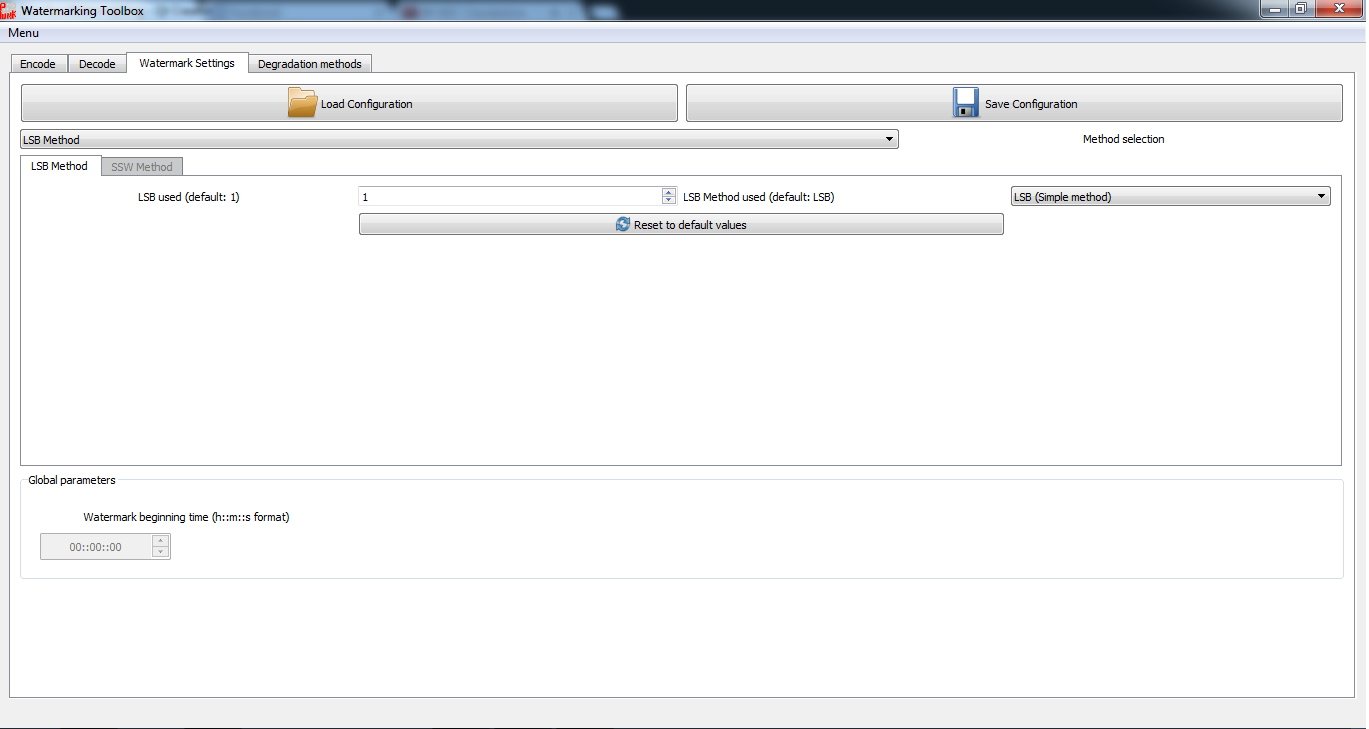
\includegraphics[scale=0.5]{images/choix.png}
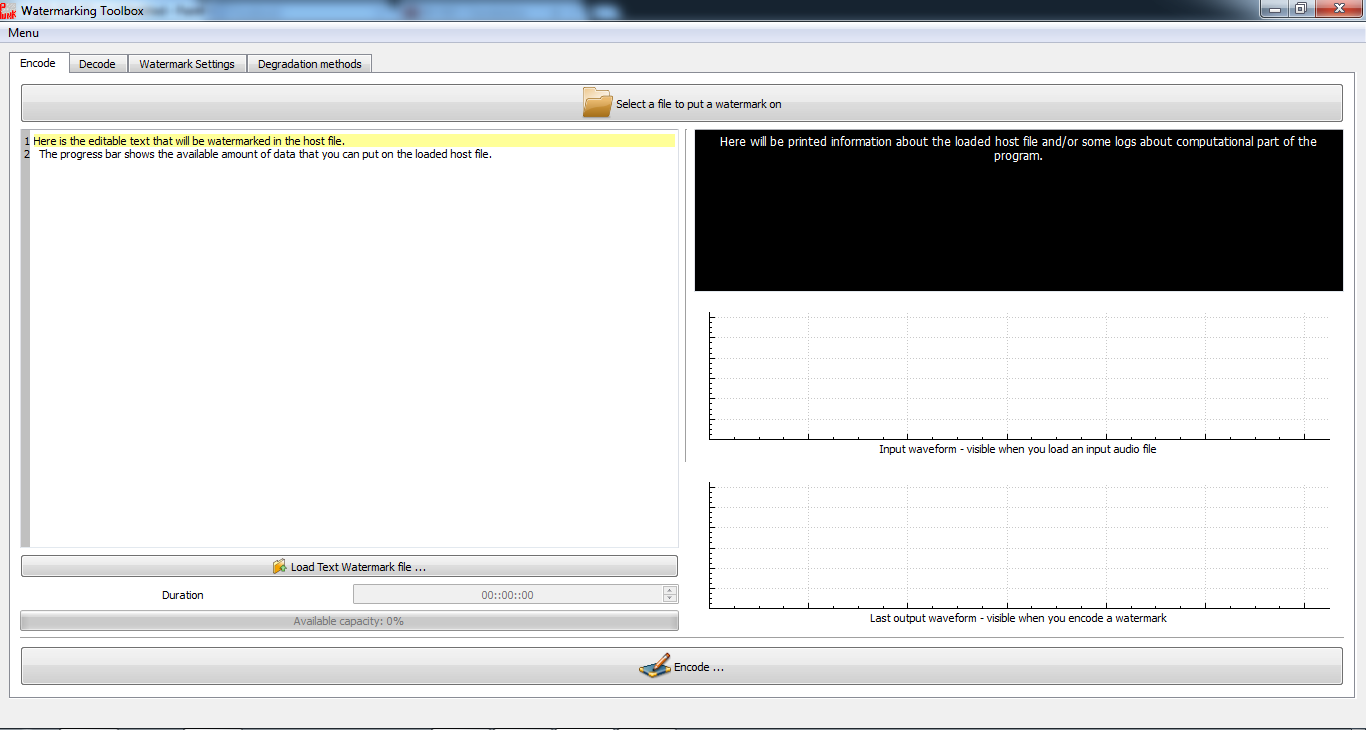
\includegraphics[scale=0.5]{images/encode.png}
\caption{Some screenshots of our software}
\end{figure}